\documentclass[12pt]{article}

% Package for including images
\usepackage{graphicx}
% Package for database diagrams and other diagrams
\usepackage{tikz}
% Package for hyperlinks
\usepackage{hyperref}
% Package for figure placement
\usepackage{float}

\title{FarmClash - Software Product Technical Manual}
\author{Your Name and Team Members' Names}
\date{\today}

\begin{document}

\maketitle
\tableofcontents
\newpage

\section{Introduction}
\subsection{Purpose}
This document serves as the comprehensive manual for the Software Product, detailing the design, database schema, and functionality to assist developers, testers, and users in understanding the system.

\subsection{Scope}
Include information about the scope of this manual, detailing the software product's intended functionalities and the audience for this document.

\section{System Overview}
Describe the overall design of the program, including a high-level architecture diagram and a description of the main components.

\section{Database Design}
\subsection{Database Schema}
The database schema is designed to support a farming simulation game, featuring users, farms, buildings, crops, and other elements essential for gameplay. The schema consists of several interconnected tables, each serving a specific purpose within the game's ecosystem. Key relationships between tables are established through foreign keys, ensuring data integrity and facilitating complex queries that drive game mechanics.

% Including an image (Your diagram)
\begin{figure}[H]
 \centering
 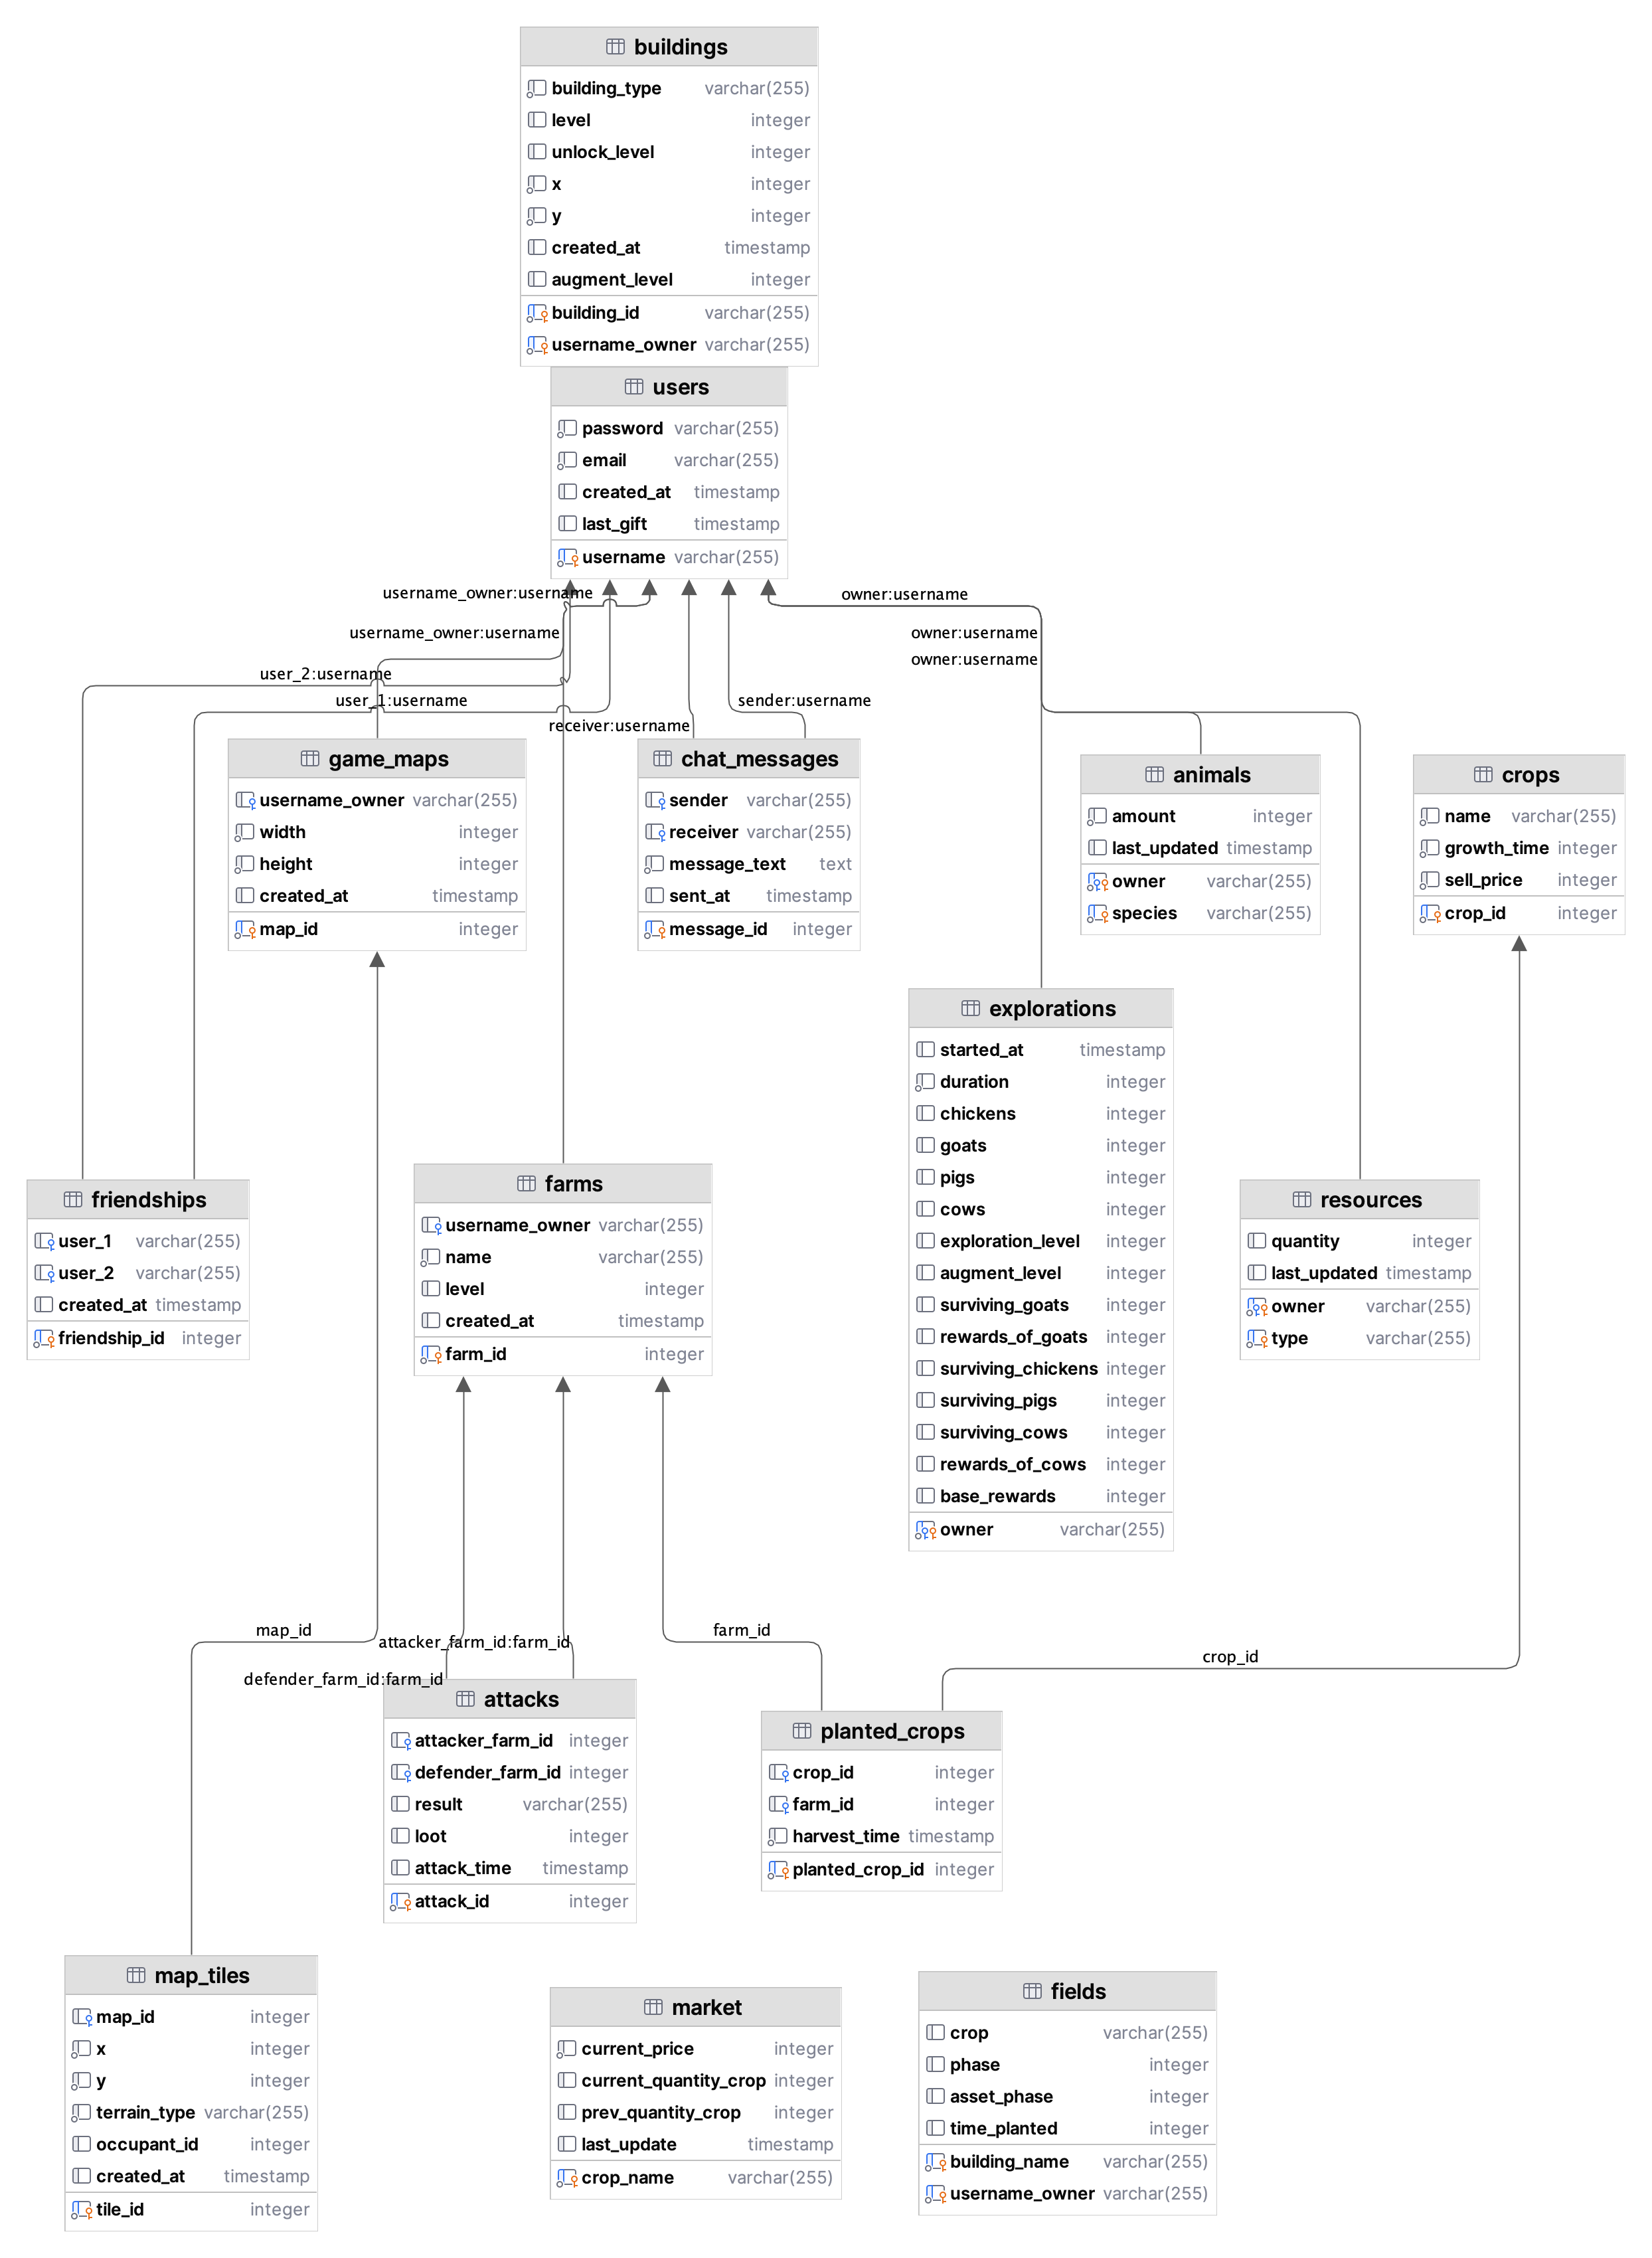
\includegraphics[width=0.8\textwidth]{img/db-diagram.png}
 \caption{Database schema diagram}
\end{figure}


\subsection{Table Descriptions}

\subsubsection{Users Table}
The users table stores information about players, including their username, password, email, and account creation date. Each user is uniquely identified by their username.

\subsubsection{Farms Table}
This table represents the farms owned by users. It includes a unique ID for each farm, the username of its owner (linked to the users table), the farm's name, its level, and the creation date.

\subsubsection{Buildings Table}
The buildings table tracks buildings on each farm, identified by a unique building ID. It stores the farm ID (linked to the farms table), the type of building, its level, and the creation date.

\subsubsection{Crops Table}
This table lists all available crop types in the game, including their name, growth time, and sell price. Each crop type is uniquely identified by a crop ID.

\subsubsection{Planted Crops Table}
The planted \textunderscore crops table keeps track of crops planted on farms, including a unique ID for each planted crop, the crop ID (linked to the crops table), the farm ID (linked to the farms table), and the harvest time.

\subsubsection{Market Table}
(Optional) The market table is designed for dynamic pricing of crops. It includes a market ID, crop ID (linked to the crops table), the current price of the crop, and the last update time.

\subsubsection{Resources Table}
This table tracks various resources owned by users, such as money or inventory items. It includes a resource ID, the owner's username (linked to the users table), the type of resource, and the quantity.

\subsubsection{Attacks Table}
(If implementing the attack feature) The attacks table records attacks between farms, including the attack ID, attacker and defender farm IDs (linked to the farms table), the result of the attack, the loot stolen, and the attack time.

\subsubsection{Friendships Table}
The friendships table tracks friendships between users, including a friendship ID, the usernames of the friends (linked to the users table), and the creation date of the friendship.

\subsubsection{Chat Messages Table}
This table stores chat messages sent between users, with a message ID, sender and receiver usernames (linked to the users table), the message text, and the time sent.

\subsubsection{Game Maps Table}
The game \textunderscore maps table stores information about game maps owned by users, including a map ID, the owner's username (linked to the users table), the map's width and height, and the creation date.

\subsubsection{Map Tiles Table}
This table tracks individual tiles within game maps, including a tile ID, the map ID (linked to the game \textunderscore maps table), the x and y coordinates of the tile, the terrain type, an optional occupant ID, and the creation date.

\subsection{Table Descriptions}
For each table in the database, provide a detailed description, including the purpose of the table, a description of each field, and the relationships to other tables.

\section{Functionality Description}
\subsection{Login Feature}
Detail the implementation of the Login feature, including any relevant code snippets, algorithms, or flowcharts.
% Example for including a code snippet
% \begin{verbatim}
%   Code snippet here
% \end{verbatim}

\subsection{Other Features}
Describe other features of the software, following the same format as the Login feature section. Include diagrams or flowcharts if applicable.

\section{Development and Implementation}
Discuss how the project was developed and implemented, emphasizing the involvement of each team member in various phases such as coding, testing, and documentation.

\section{Conclusion}
Summarize the key points of the manual and the software product's capabilities.

\end{document}
